\documentclass[compress]{beamer}
\usepackage{euscript,amsmath,amssymb,amsfonts,amsthm,epsfig,subfigure,color,graphicx,media9}
\usepackage[utf8]{inputenc}
\usepackage[french]{babel}
\usepackage[T1]{fontenc}
\usepackage{pgfgantt}
\usepackage{pgf,csquotes}
\usepackage{tabularx}
\usepackage{tikz}
\usetikzlibrary{fit,arrows,positioning}
\newsavebox{\mysavebox}

% \definecolor{blue}{rgb}{51,131,255}
%
%\usepackage[autolinebreaks,useliterate]{mcode}

% \usepackage{letltxmacro}
% \LetLtxMacro\olditemize\itemize
% \LetLtxMacro\oldenumerate\enumerate

\graphicspath{{../poster/figures/}{../paper/figures/}}

\usepackage[doi=false,
            isbn=false,
            url=false,
            mincitenames=20,
            maxcitenames=20,
            firstinits=true,
            bibstyle=authoryear,
            backend=biber,
            style=authoryear]{biblatex} %, backend=bibtex
\AtEveryCitekey{%\clearfield{title}
    \scriptsize
    \clearfield{note}
    \clearfield{pages}
    \clearfield{volume}%
    \clearfield{number}
    \clearlist{location}
    \clearlist{publisher}
    \clearname{editor}}
\renewcommand*{\multicitedelim}{\\}
%
%
\addbibresource{../poster/bib.bib}
\addbibresource{../paper/refs.bib}
% \addbibresource{bib/bib.bib}
% \addbibresource{bib/references.bib}
% \addbibresource{bib/journals.bib}
% \addbibresource{bib/conferences.bib}
% \addbibresource{bib/software.bib}

\usepackage{beamerthemedefault, multimedia, wasysym, amssymb, kpfonts}

\useoutertheme{smoothbars}
\useinnertheme[shadow=true]{rounded}
\setbeamercovered{transparent}
\setbeamertemplate{navigation symbols}{}
\setbeamertemplate{footline}[frame number]
\setbeamerfont{footline}{size=\fontsize{7}{11}\selectfont}
%\setbeamertemplate{itemize items}{$\multimapdotinv$}
%\setbeamertemplate{itemize items}{\textbf{$\strictfi$}}
\setbeamertemplate{enumerate items}[circle]
\setbeamertemplate{section in toc}[circle]
%\useoutertheme{infolines}
\setbeamercolor{block title}{bg=green}

\definecolor{violet}{rgb}{0.8, 0.6, 0.8}
\definecolor{green}{rgb}{0.8 ,.9, 0.8}
\definecolor{blue}{rgb}{0.3, 0 ,0.6}

\newcommand{\includesound}[1]{
\includemedia[
  addresource=#1,
  flashvars={
    source=#1
   &autoPlay=true
  }
]{\structure{\includegraphics[keepaspectratio,width=.5cm]{figures/play}}}{APlayer.swf}
}

% footnote without numbers
\let\oldfootnote\footnote
\renewcommand\footnote[1]{\let\thefootnote\relax%
\oldfootnote{#1}}

\newrobustcmd*{\footfullcitenomark}{%
  \AtNextCite{%
    \let\thefootnote\relax
    \let\mkbibfootnote\mkbibfootnotetext}%
  \footfullcite}

  \defbeamertemplate*{footnotetext}{default}{%
  %\parindent 1em\noindent%
  \raggedright
  %\hbox to 1.8em{\hfil\insertfootnotemark}%
  \insertfootnotetext\par}
%
\newrobustcmd*{\footfullcitenomarkleft}{%
  \AtNextCite{%
    \setbeamertemplate{footnote}{\usebeamertemplate{footnotetext}}%
    \let\mkbibfootnote\mkbibfootnotetext}%
  \footfullcite}

% title, url, authors, extensions
\newcommand\citenote[4]{\footnote{#3 \href{#2}{\structure{#1}} #4}}



\setbeamertemplate{itemize item}{\textrm{--}}

% \defbeamertemplate{description item}{align left}{\insertdescriptionitem\hfill}
% \setbeamertemplate{description item}[align left]

%\usecolortheme[named=purple]{structure}

\title[]{\LARGE \bf Bandwidth extension of musical audio signals with no side information using dilated convolutional neural networks}

\author{Mathieu Lagrange, F\'elix Gontier}

\institute[]
{
LS2N, CNRS, Centrale Nantes \\

\includegraphics[height=1.5cm]{logoCnrs}
}

\date[]{31 Mars 2020}

\logo{
\includegraphics[height=.6cm]{logoCnrs}}

\begin{document}

\tikzstyle{mystyle}=[
nonterminal/.append style={join=by ->},
tip/.style={->,shorten >=1pt},every join/.style={rounded corners},
terminal/.style={
% The shape:
rectangle,minimum size=6mm,rounded corners=1mm,
% The rest
very thick,draw=black!50,
top color=white,bottom color=black!10,
font=\ttfamily},
point/.style={circle,fill=black,minimum size=2pt},
%every node/.style=draw,
line/.style ={draw, thick, -latex',shorten
  >=2pt}]

  \AtBeginSection[]{
    \begin{frame}
    \vfill
    \centering
    \begin{beamercolorbox}[sep=8pt,center,shadow=true,rounded=true]{title}
      \huge \bf
      \secname\par%
    \end{beamercolorbox}
    \vfill
    \end{frame}
  }

% Update itemize to have a default overlay
%\renewcommand{\itemize}[1][<+(1)->]{\olditemize[#1]}
%\renewcommand{\enumerate}[1][<+(1)->]{\oldenumerate[#1]}

%\includeonlyframes{current}

\frame{\titlepage \thispagestyle{empty}}

% show section lists
%\begin{frame}{Agenda} \tableofcontents \end{frame} % [pausesections]

\begin{frame}{Introduction}
\only<1>{
  Bandwidth extension is the process of generating lost high frequencies of an audio signal given some prior knowledge which can be :
  \begin{itemize}
    \item the low frequency content
    \item some side information computed using knowledge of the high frequency content
    \item some generic knowledge of the spectral properties of the high frequencies. This knowledge can be encoded by experts or \structure{computationally learned}.
  \end{itemize}}
\only<2>{%\centering 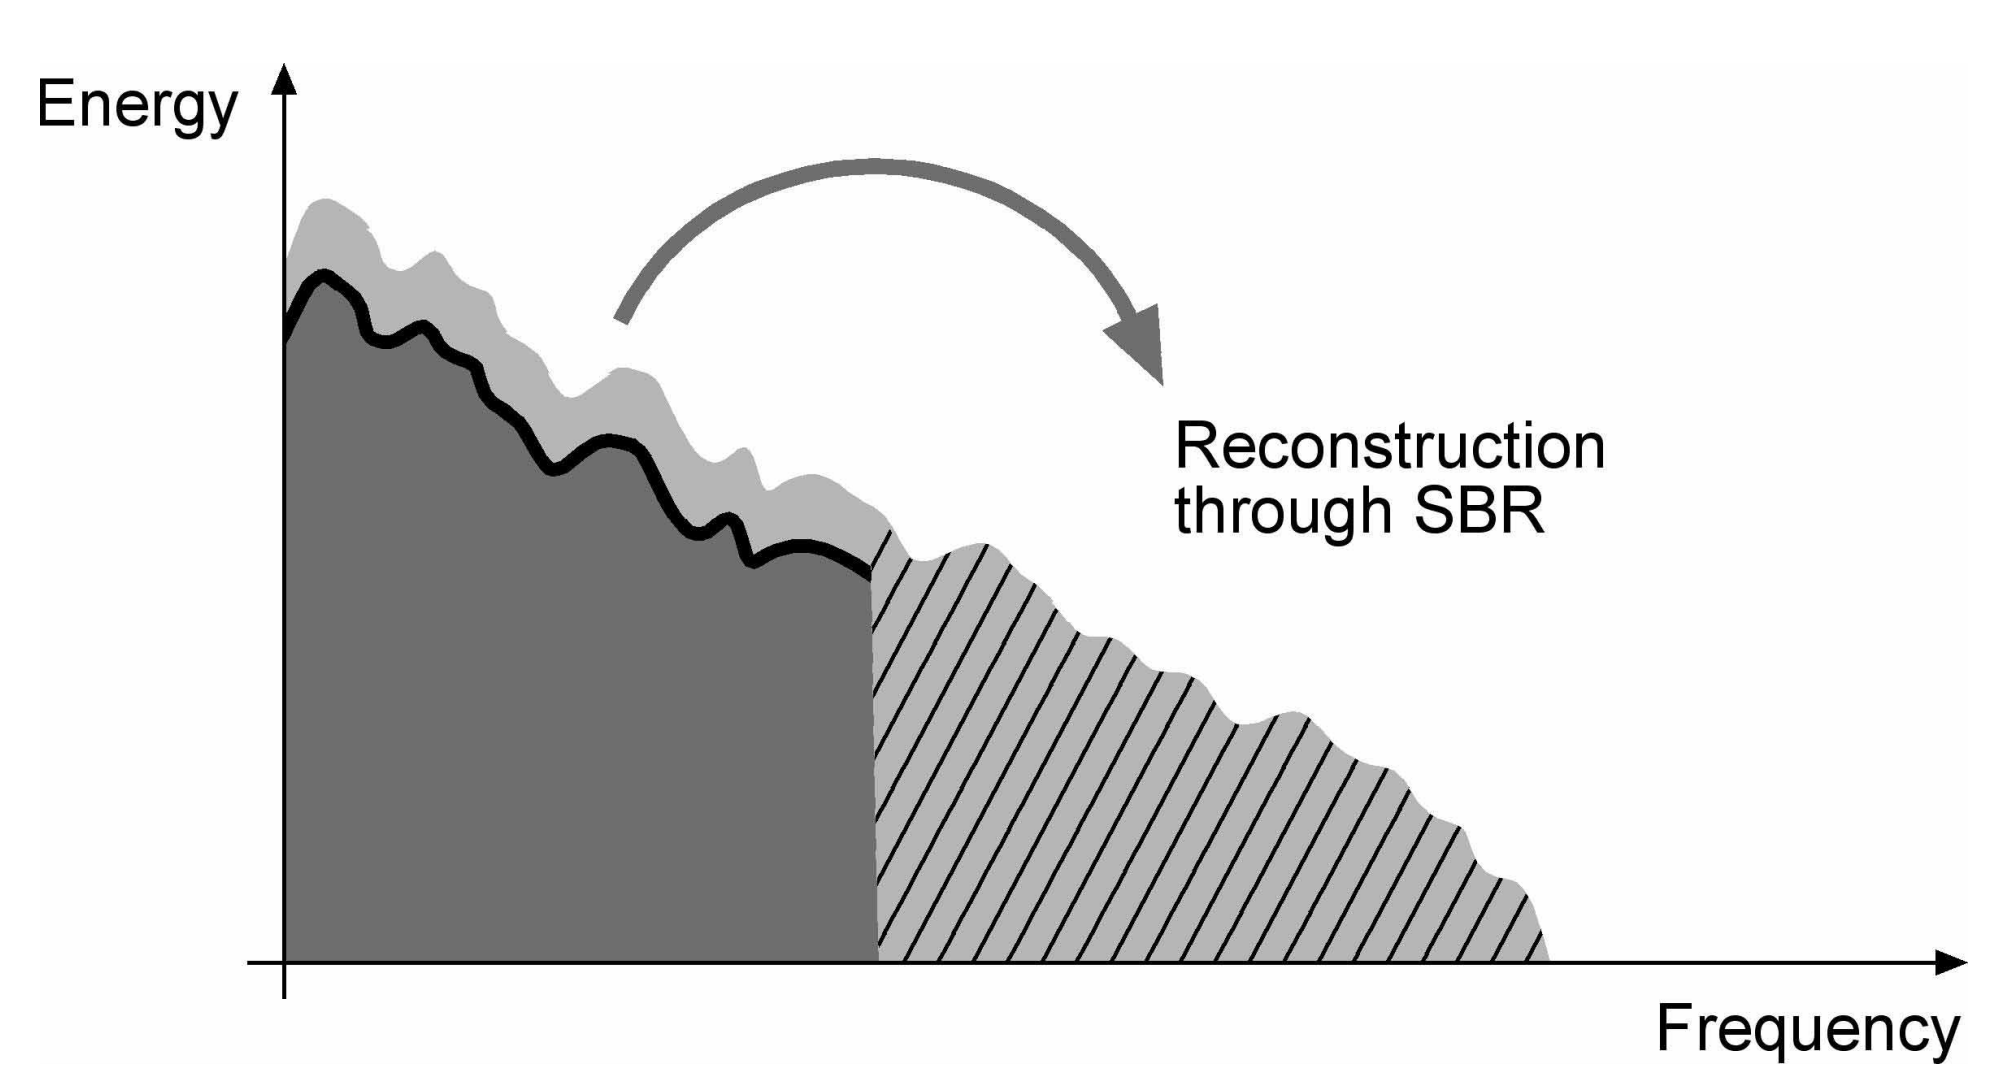
\includegraphics[width=.9\linewidth]{sbr}
sbr\\
Principle of Bandwidth Extension (fig from \footfullcitenomarkleft{dietz2002spectral}).}
\end{frame}




\section{Background}

\begin{frame}{Previous work}
  \begin{itemize}
    \item \textbf{Spectral band replication (SBR)$^*$}: M. Dietz, L. Liljeryd, K. Kjorling, and O. Kunz. "Spectral band replication, a novel approach in audio coding". In {\em Audio Engineering Society Convention}, 2002.
    \item \textbf{Non-negative matrix completion (NMC)}: D. Sun and R. Mazumder. Non-negative matrix completion for bandwidth extension: A convex optimization approach. MLSP, 2013.
    \item \textbf{Autoencoders$^*$}: M.~Miron and M.~E.~P. Davies. High frequency magnitude spectrogram reconstruction for music
      mixtures using convolutional autoencoders. DAFx, 2018.
    \item \textbf{Sample based}: A. Gupta, B. Shillingford, Y. Assael, and T. Walters. Speech bandwidth extension with wavenet, 2019.
  \end{itemize}
  $^*$ will be considered as \textbf{baselines}.
\end{frame}



\section{Model}

\begin{frame}{Proposed approach}

  \begin{itemize}
    \item The proposed approach operates on the magnitude spectrogram.
    \item From a given matrix encoding the low frequencies, the system predicts the corresponding high frequencies
    \item This prediction is done considering some prior knowledge that is learned.
    \item In the experiments, the phase spectrogram of the high frequencies needed for sample reconstruction is whether assumed be known or heuristically defined.
  \end{itemize}
\end{frame}

\begin{frame}{Proposed model}
  \only<1>{\begin{enumerate}
    \item $L$ layers followed by rectified linear units (ReLU) activations
    \item The number of output convolution channels $C$ is the same for all hidden layers
     \item Convolution kernels also share the same size $(K_t, K_f)$ in the time and frequency dimensions respectively
     \item padding by replicating their boundary values depending on the kernel size
     \item a fixed dilation ratio $D$ is used in the frequency dimension for hidden layers, and no dilation is used in the input and output layers of the network
  \end{enumerate}}
\only<2>{
 \begin{center}
    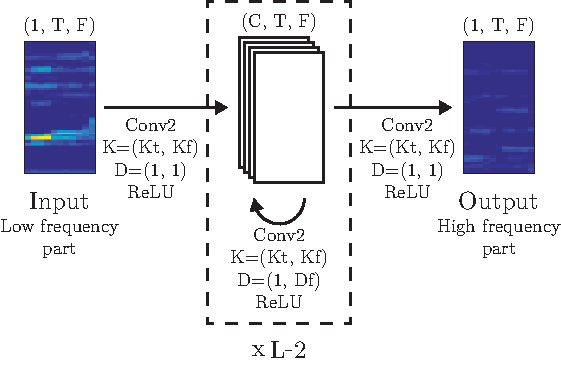
\includegraphics[width=.9\linewidth]{mdl}

Proposed deep convolutional neural network architecture for bandwidth extension.
\end{center}
}
\end{frame}

\begin{frame}{A word on dilation}
  \only<2>{
  From a signal processing standpoint,
  \begin{itemize}
    \item this procedure is equivalent to applying the convolution on a down-sampled version of the input.
    \item As a result each hidden layer increases the receptive field by $D(K-1)$ frequency bins
    \item compared to $K-1$ without dilation.
  \end{itemize}
}
\only<1>{
  \begin{center}
%  \includegraphics[width=.8\linewidth]{dilation2}
dilation2
Dilation can be viewed as a convolution on a downsampled version of the input (fig from \footfullcitenomarkleft{tan2018gated}).
  \end{center}}
\end{frame}

\section{Experimental protocol}

\begin{frame}{Datasets}
\begin{enumerate}
  \item \textit{medley-solos-db}: 18 hours, monophonic
  \item \textit{gtzan}: 8 hours, polyphonic
\end{enumerate}
Pre-processing:

\begin{enumerate}
  \item resampling to $8$kHz
  \item short-term Fourier transform with frame size of $256$ samples, hop size of $128$ samples and a Hann window.
  \item "textures" of $10$ frames, processed as individual examples.
\end{enumerate}
\end{frame}

\begin{frame}{Metrics}
Three metrics are considered:
\begin{enumerate}
  \item \textbf{Spectral loss} : the loss used to optimize the network
  \item \textbf{SRR} : signal to reconstruction ratio computed in the time domain
  \item \textbf{$PSM_t$} : perceptual similarity measure from PEMO-Q \footfullcitenomarkleft{huber2006pemo}
\end{enumerate}
\end{frame}

\begin{frame}{Anchors and baselines}

Two anchors are considered:
\begin{enumerate}
  \item \textit{oracle}: the predicted magnitude in the high frequencies are the actual ones
  \item \textit{null}: the predicted magnitude in the high frequencies are set to zero
\end{enumerate}

Three baselines are considered:
\begin{enumerate}
  \item \textit{sbr}: crude implementation of the SBR technique
  \item \textit{cnn bottleneck}: reimplementation of bottleneck autoencoder architecture proposed by Miron \& al
  \item \textit{cnn stride2}: reimplementation of a strided autoencoder architecture proposed by Miron \& al \footfullcitenomarkleft{miron2018high}
\end{enumerate}
\end{frame}

\section{Experiments}

\begin{frame}{Inspection of predicted high frequencies}
  \centering
\only<1>{
    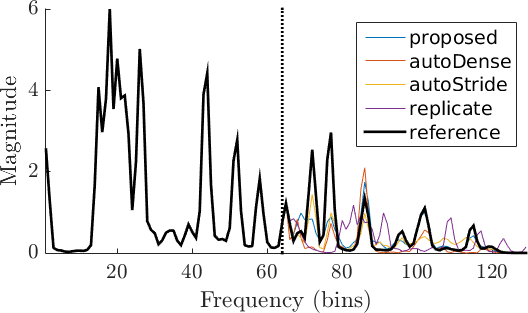
\includegraphics[width = .9\columnwidth]{solos_1141Legend.png}

  The proposed model handles correctly the harmonic structures (\textit{medley-solos-db} dataset).
  }
  \only<2>{
      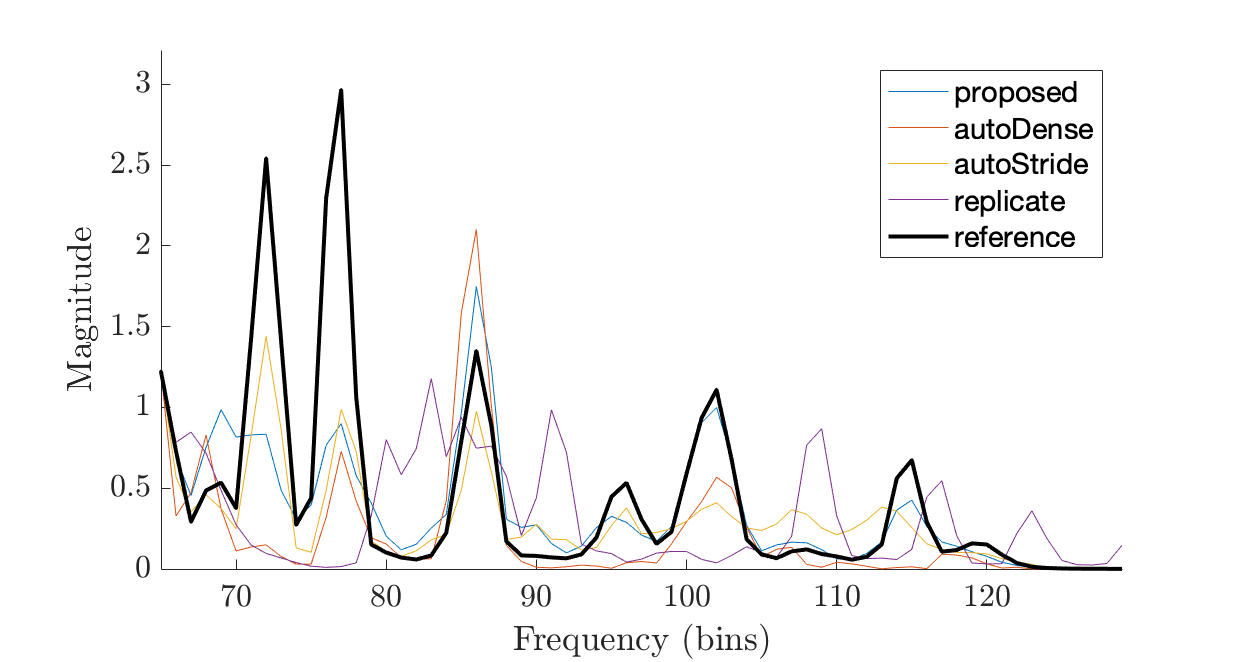
\includegraphics[width = .9\columnwidth]{solos_1141Zoom.png}

    The proposed model handles correctly the harmonic structures (\textit{medley-solos-db} dataset).
    }
  \only<3>{
    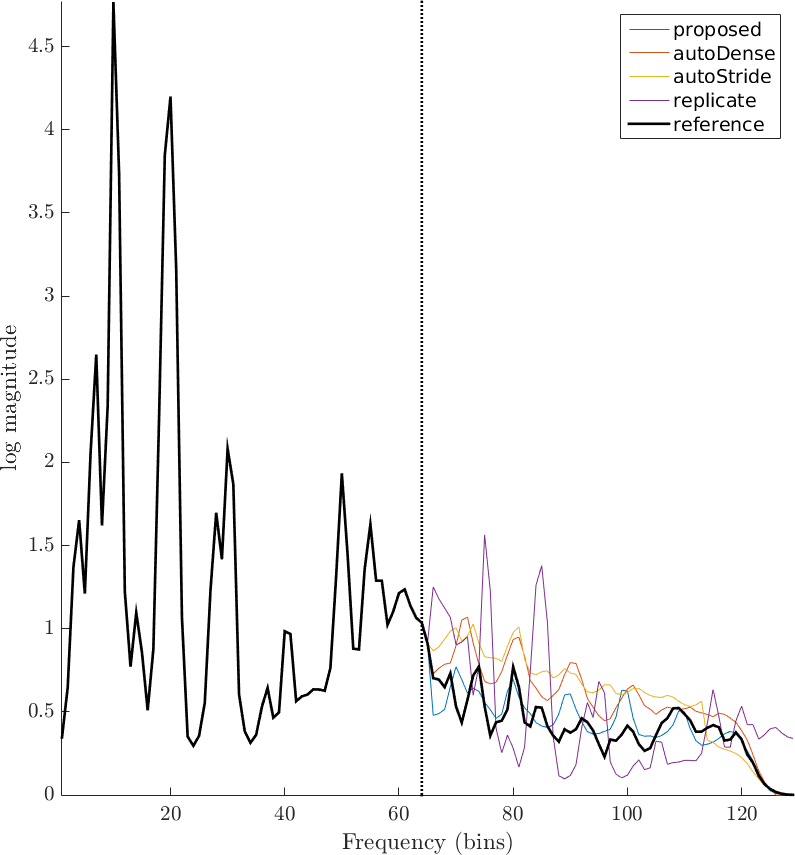
\includegraphics[width = .9\columnwidth]{gtzan_1120.png}

    The proposed model handles correctly the average magnitude of complex spectral shapes (\textit{gtzan} dataset).
    }
    \only<4>{
      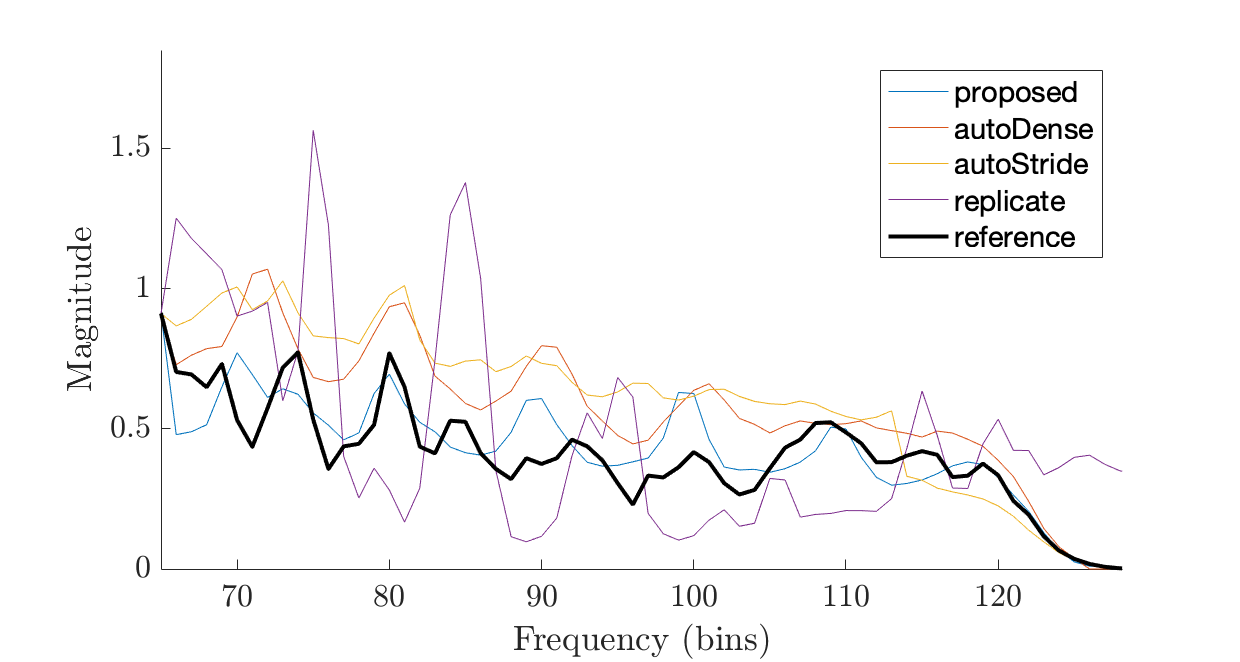
\includegraphics[width = .9\columnwidth]{gtzan_1120Zoom.png}

      The proposed model handles correctly the average magnitude of complex spectral shapes (\textit{gtzan} dataset).
      }
\end{frame}

\begin{frame}{Impact of dilation on the spectral loss}
  \begin{center}
\begin{tabular}{llcc}
$L$ & dilation ($D$) & \textit{medley-solos-db} & \textit{gtzan} \\
\hline
5 & 1 & 0.240 $\pm$0.013 & 0.110 $\pm$0.017 \\
6 & 1 & 0.231 $\pm$0.016 & 0.107 $\pm$0.021 \\
7 & 1 & 0.226 $\pm$0.016 & 0.105 $\pm$0.021 \\
5 & 2 & 0.228 $\pm$0.015 & 0.102 $\pm$0.019 \\
6 & 2 & 0.225 $\pm$0.019 & 0.102 $\pm$0.022 \\
7 & 2 & 0.218 $\pm$0.019 & 0.102 $\pm$0.022 \\
% 5 & 3 & - $\pm$- &     - $\pm$- \\
% 6 & 3 & - $\pm$- &     - $\pm$- \\
% 7 & 3 & 0.103 $\pm$0.022 &     - $\pm$- \\
\end{tabular}

Spectral loss on the testing set for the proposed architecture with $K=17$ and $C=64$.
  \end{center}
\end{frame}

\begin{frame}{Prediction performance in terms of spectral loss}
  \begin{center}
\begin{tabular}{lcc}
method & \textit{medley-solos-db} & \textit{gtzan} \\
\hline
proposed & 0.225 $\pm$0.019 & 0.102 $\pm$0.022 \\
cnn bottleneck & 0.241 $\pm$0.011 & 0.107 $\pm$0.017 \\
cnn stride2 & 0.228 $\pm$0.013 & 0.110 $\pm$0.017 \\
\end{tabular}
\end{center}
\end{frame}

\begin{frame}{Perceptually motivated objective performance ($PSM_t$) using the mirror phase estimate}
  \begin{center}
  \begin{tabular}{lcc}
  method & \textit{medley-solos-db} & \textit{gtzan} \\
  \hline
  null & 90.9 $\pm$1.6 & 89.7 $\pm$2.3  \\
  replicate & 86.5 $\pm$1.4 & 88.4 $\pm$1.8 \\
  \hline
  cnn bottleneck & 86.6 $\pm$1.5 & 91.3 $\pm$1.8 \\
  cnn stride2 & 86.9 $\pm$1.3 & 90.4 $\pm$2.1 \\
  \hline
  proposed & 87.5 $\pm$1.4 & 91.5 $\pm$1.8 \\
  \hline
  oracle & 97.2 $\pm$0.3 & 97.2 $\pm$0.6 \\
\end{tabular}
  \end{center}
\end{frame}

\begin{frame}{Forthcoming Research}
\begin{enumerate}
  \item \textbf{advanced phase estimators}
  \item \textbf{mismatch between training and testing audio material}
  \item \textbf{creative use} : predicting the high frequency spectra of a 'pop' song using network trained on 'country' songs may be of creative interest, to explore the yet to be defined notion of \textbf{musical style transfer}.
\end{enumerate}
\end{frame}

% \begin{frame}{References}
% \bibliographystyle{../paper/IEEEbib} % Plain referencing style
% \bibliography{../poster/bib,../paper/refs}
% \end{frame}

\end{document}
